\chapter{Background}
\label{chapt:Background}
Following is an outline of the different models and extensions found in literature on access Control.
We focus on Role based authorization control (RBAC) and the more general Attribute based access control (ABAC) models, RBAC extensions, such as constraints and hierarchy, and models that are similar to them such as Task RBAC.
We also look at hybrid models that have gained attention recently such as attribute enhanced role based access control (AERBAC).
The other 2 big models as often found in literature, as mentioned by Ryan Ausanka-Crues in Methods for Access Control: Advances and Limitations\cite{SurveyAC2}, Yogita S. et al. their survey on access control models and application\cite{SurveyAC} and  Romuald Thion on Access control models\cite{MACDAC}, will not be handled in this thesis.
These are the discretionary access control (DAC) model  where owners of resources are responsible for access control and the mandatory access control (MAC) model where we work with different clearance levels.
From the following models we make 2 into prototypes in the application of our case study, these can then be used to run various scenarios and gather metrics to determine which one model scores best in which situation.

\section{Role based access control (RBAC)}
Following is a short overview of what RBAC exactly is, this is based on reports of the American National Institute of Standards and Technology(NIST), these can be consulted for a more in depth view on RBAC\cite{Overview1}.
The idea of using RBAC is that instead of giving permissions to every user of the system individually, the notion of roles is introduced.
Under these roles we can bring together multiple users that all have the same set of permissions.
This with the intention of making management of users less error prone because now the people managing this only have to assign permissions to roles instead of individual users.
This opposed to manually assigning and withdrawing every single permission per user on a change in permissions.
Users can be both humans or other machines.

\begin{figure}[ht]
    \centering
    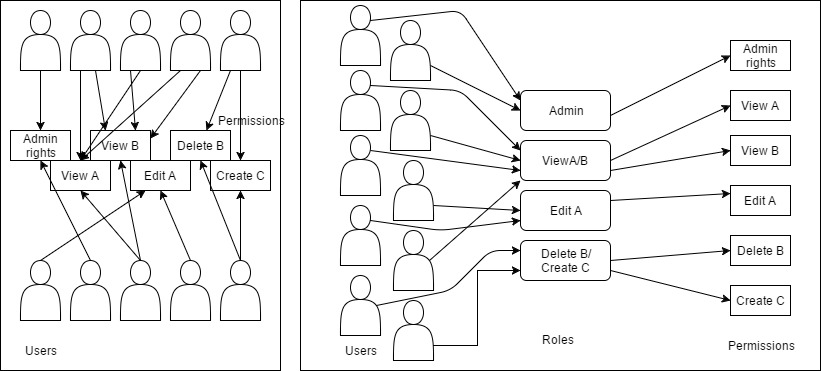
\includegraphics[width=0.9\textwidth, height=0.50\textwidth]{Img/self/RBACvsNonRBAC.jpg}
    \caption{Compares managing users and permissions, left without roles, right with the use of roles.}
\end{figure}
The basic building blocks of the role based access control model are the following (based on the list given in The NIST model for RBAC : Towards a unified standard \cite{Overview1}) :
\begin{itemize}
    \item Each user is assigned to one or more possible roles
    \item Each role gets permissions assigned to them, this number of permissions can vary from none to multiple
    \item A permission is a mapping from an operation to an object
    \item Different roles can have overlapping permissions
    \item Users get the permissions of the roles they belong to, we can use sessions to restrict the active roles a user has at a time and allow them to switch between their different roles
    \item It should be easy to get an overview of users/roles and roles/permissions relations
\end{itemize}
Below is the scheme of the relationship between the different building blocks for the role based access control system. 
We can see that a user can have multiple roles and that roles can be assigned to multiple users as depicted by the double arrow.
The same goes for roles and permission, permissions exist of out combinations between objects and actions.
A user has a single session which in turn can be related to multiple roles, these are the active roles for that user.
In our implementation we limit this to one role in order to maximize conformity with the principle of least privilege. 
This means the user can only access objects with the permissions of one role and not all the other roles they have assigned, but do not need the permissions of at that time, limiting access to the minimal level of accessibility that allows normal functioning of that role. 

\begin{figure}[ht]
    \centering
    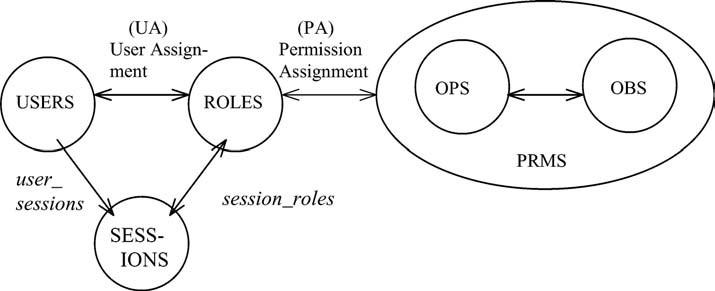
\includegraphics[width=0.7\textwidth, height=0.4\textwidth]{Img/standard/coreRBAC.jpg}
    \caption{Core RBAC scheme, adapted from the NIST standard report\cite{Standard}}
\end{figure}

\subsection{Hierarchical RBAC}
The first extension that can be done on the role based access control model is that of introducing hierarchy.
We give the basics of this extension, for a more in depth view look at the NIST standard\cite{Hierarch},\cite{Standard}.
The idea here is that instead of having multiple individual roles we create a hierarchy of roles.
In this hierarchy a role can get all the permissions from the role it inherits from and have its own permissions assigned to it that the role it inherited from did not have.
While hierarchies can be done in any arbitrary form (general hierarchy), there is also the limited hierarchy which restricts the structure to just trees.
This means that multiple inheritance, a role that derives from multiple other roles, is not allowed for limited hierarchy, but it is for general hierarchy.
Following is the scheme for hierarchical role based access control, it is similar to the normal role based access control one with the addition of a relationship between roles where a role can inherit from multiple roles and a role can be inherited by multiple roles.

\begin{figure}[ht]
    \centering
    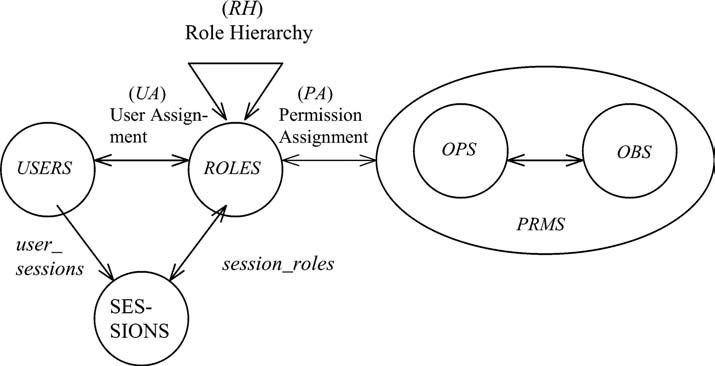
\includegraphics[width=0.7\textwidth, height=0.40\textwidth]{Img/standard/hierarchRBAC.jpg}
    \caption{Hierarchical RBAC scheme, adapted from the NIST standard report\cite{Standard}}
\end{figure}

\textbf{Example} In the image below we can see that we have 4 roles available, User, Employee, Consultant and supervisor. 
All of these roles have their associated permissions A, B, C, D and E.
Since user has the permission A associated with it and all other roles inherit from the User role this means that all other roles also get permission A associated with them.
This means that the supervisor role has permissions A, B, C and D, A inherited from User, B and C inherited from employee and D from its own role. 
The consultant role only has permissions A from inheriting from User and its own permission E.

\begin{figure}[!h]
    \centering
    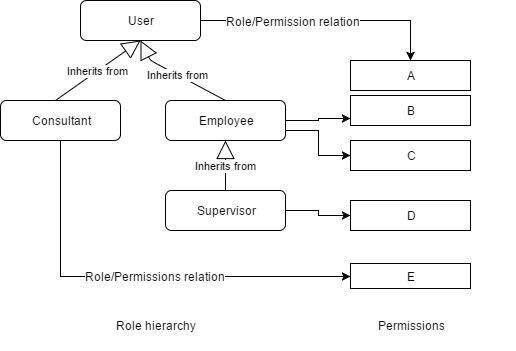
\includegraphics[height=0.55\textwidth,width=0.8\textwidth]{Img/self/ExampleHierarch.jpg}
    \caption{Hierarchical RBAC example}
\end{figure}

\subsection{Constraint based RBAC}
Another extension on the role based access control model makes use of constraints as described in A framework for en-forcing constrained RBAC policies\cite{Constraint}.
Both the constraint and hierarchical extension to role based access control can be used individually on top of the basic model or in combination.
The main idea is that by making use of constraints we can limit human errors made by the administrators that go against rules set by the company.
This also prevents abuse, as well as introduces a way to enforce more specific business rules. 
The biggest reason for using constraints however is to enforce the principle of separation of duty, where we can make it impossible that a single user with all the needed rights can perform a task without the involvement of a second user with the needed rights.
\\
\\
This principle of separation of duty can be enforced in two ways with constraints:

\begin{enumerate}
    \item Static separation of duty, this type of constraint does not depend on any state of an object. 
    
    \textbf{Example} We have 2 specific roles that need to sign off on a task before it can continue.
    With static separation of duty we make it impossible for the manager to assign both of these roles to a single user. 
    This means that we need 2 different users with 2 different roles to sign off on a given task before it can continue.
    
    \item Dynamic separation of duty, this type of constraint depends on the current state of an object.
    
    \textbf{Example} We have a constraint that requires two different people to sign off for a certain action to be done. 
    Even though one person may have all the needed permissions, they can still only do one sign off and someone else with the correct permissions is needed to do the second sign off.
    We look at the state of the system (who has already signed off) to see if a user is allowed to be the second person to sign off.
    
    \textbf{Example} Another example would be the constraint of there may only be 1 CEO at a time, which also depends on the state of the management system.
\end{enumerate}
\\
\\
The image below is the same one as used for hierarchy but now we also have added the blocks Static separation of duty(SSD) and dynamic separation of duty (DSD).
The Static block has a relation with the existing roles in the system and the assignment of roles to users, the dynamic block has a relation with the active sessions to roles relationship.
The dynamic constraints are placed on the sessions and are determined on the current session status.

\begin{figure}[ht]
    \centering
    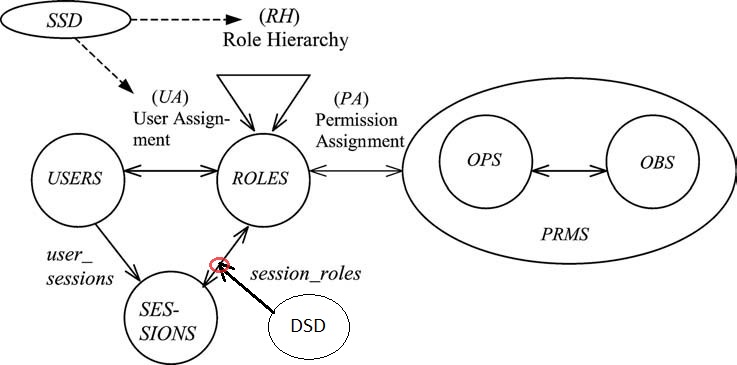
\includegraphics[width=0.7\textwidth, height=0.40\textwidth]{Img/standard/combinedConstraint.jpg}
    \caption{Constrained RBAC scheme, adapted from the NIST Standard \cite{Standard}}
\end{figure}

\section{Attribute based access control (ABAC)}
 Attribute based access control (ABAC) is a more general approach to role based access control. 
 While role based access control only focuses on the user roles, attribute based access control makes use of multiple attributes.
 These attributes can be on users, objects, actions or even environmental.
 By the combination of attributes a user has and the attributes an object has we can decide if that user can access that given object.  
\\
\\
The building blocks for attribute based access control as described in A Unified Attribute-Based Access Control
Model Covering DAC, MAC and RBAC\cite{ABAC2} and Guide to Attribute Based Access Control (ABAC) Definition and Considerations\cite{ABAC} are the following:
\begin{description}
    \item [Attribute]Attributes represent the characteristics of those objects/users/action/environments they are associated with.
    Users, actions and objects can have attributes, apart from this we can also have environmental attributes.
    We can use the value of these attributes to determine if access is granted or not.
    \item [Object] Objects are the things we want to access. Each object has attributes for example when it was created, who created it, what research group it belongs too, etc. 
    \item [User] A user of the system, can be both a machine or human, the user requests access to certain object. Each user also has its own attributes such as the user name, email, date of registration etc.
    \item [Policy] A policy can use the different available attributes from users, objects, the environment and actions to decide on whether or not a user can access a certain resource with that action under those circumstances.
    A policy can be both positive and negative, with negative ones taking priority.
    If you meet a negative policy you are not allowed to perform the action no matter how many positive ones you meet.
    A policy example would be that all users that registered before 1/01/2000 are allowed to access the files created in the 90's.
    \item [Operation] Can be done on an object, these operations can be database CRUD actions as well as execution of functions, actions can also have certain attributes.
    \item [Environmental condition] Do not depend on user and object, this condition is purely dependant on the environment, for example the air pressure in a room or the current time.
\end{description}
\textbf{Example} Using the image below we see that there are 2 users, a senior developer and a normal developer this role is an attribute, both users also have a name as attribute.
There are 3 objects, source code with a critical level attribute, source code with a normal level attribute and a payroll object which has the name of the user it belongs to as an attribute.
3 policies have been defined on the system.
If the user named Al tries to access the payroll his is not allowed since the its the payroll of Bert so only Bert can access it.
Al who is a senior developer can access both the source code of critical and normal level, Bert however being only a developer can only access the source code of normal type.

\begin{figure}[ht]
    \centering
    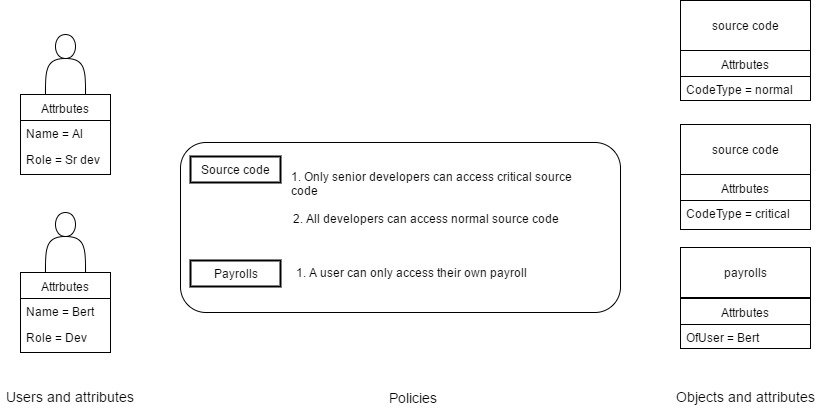
\includegraphics[height=0.45\textwidth, width=0.75\textwidth]{Img/self/ABACExample.jpg}
    \caption{ABAC example}
\end{figure}
The proposed architecture for building  attribute based  access control model as presented in Guide to Attribute Based Access Control (ABAC) Definition and Considerations \cite{ABAC} makes use of the following 4 components:
\begin{description}
    \item [PEP] The policy enforcement point, this point intercepts a call for access and asks the PDP if that user is allowed to access the demanded data.
    If the user is allowed to access it the PEP will let the call pass if not it will refuse it.
    \item [PDP] The policy decision point, this point uses all the data made available to it from a policy database and the different PIP's to make a decision for a user that wants to access certain resources.
    \item [PIP] The policy information point (or points) are databases that provide the attribute information for the different users, objects, actions and the environment to the PDP so it can make its decisions.
    \item [PAP] The policy administration point is used to edit the different policies that exist, this allows a user to add new policies and delete or change existing policies.
\end{description}
The following image illustrates their relationship with each other and the system in a visual way.

\begin{figure}[ht]
    \centering
    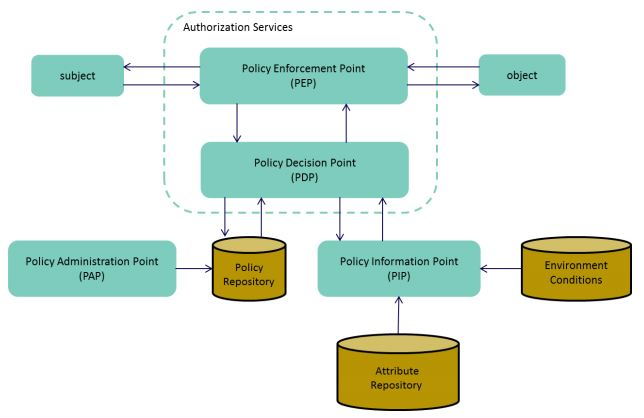
\includegraphics[width=0.75\textwidth, height=0.40\textwidth]{Img/standard/ABACArchi.JPG}
    \caption{Architecture ABAC and relation between the different points, adapted from the NIST Guide to Attribute Based Access Control (ABAC) Definition and Considerations \cite{ABAC}}
\end{figure}

\section{Attribute enhanced RBAC (AERBAC)}
Attribute enhanced role based access control is, as the name suggests, a hybrid form that combines aspects of both role based access control and attribute based access control in a single model in an effort to get the benefits of both models.
These hybrid models can include both the constraints and hierarchy extensions available for RBAC.
This can be done in multiple ways as shown by D. Richard Kuhnet et al in Adding Attributes to Role-Based Access Control\cite{Combined1}, where they sum up the different types of combinations that can be made.
Multiple hybrid versions have been proposed, such as Ting Cai et al their Hybrid attribute based RBAC model\cite{Combined2} where they split up permissions in static and dynamic permissions.
\\
\\
Another such hybrid model, which is the one we focus on, is Qasim Mahmood Rajpoot et al with their Attributes Enhanced Role-Based Access Control Model\cite{Combined3}.
This model enhances the previous handled role based access control model with conditions on the permissions, these conditions make use of different attributes.
This gives the following scheme of the different building blocks and their relationship to each-other.
We can see that on the permissions we can put a set of conditions and that objects and users have attributes related to them. 
For checking access we can also make use of environmental attributes such as current time, temperature and so on.
Using all of these attributes in the conditions we can then evaluate the condition and an allow or deny access decision, that gives access to a resource for a given user, can then be made.

\begin{figure}[ht]
    \centering
    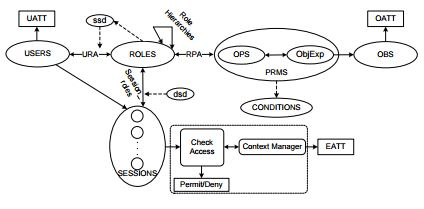
\includegraphics[width=1\textwidth, height=0.45\textwidth]{Img/self/AERBAC.JPG}
    \caption{AERBAC scheme, adapted from Enhanced Role-Based Access Control Model\cite{Combined3}}
\end{figure}
\section{Organizational units}
The idea of organizational units, as defined by M .Umar Aftab et all \cite{OU}, is that apart from only working with roles we will also work with organizational units.
This is an intermediate building block between users and roles which allows us to assign users to organizational units before giving them roles.
Like this users will already be divided on the organizational level, often departments, where already only a sub set of permissions may be applicable, this before they get roles assigned to them.
The permissions are still assigned to the roles.
Doing this allows for a finer grained access control system when dealing with very large multi departmentalized companies.
Below is an example of how the organization would look like when using permissions, roles, users and organizational units.

\begin{figure}[h]
    \centering
    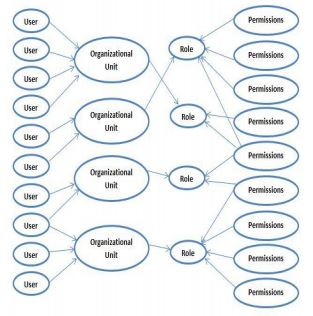
\includegraphics[width=0.75\textwidth, height=0.55\textwidth]{Img/self/OUExample.JPG}
    \caption{Overview of management using organisational units, adapted from RBAC Architecture Design Issues in Institutions Collaborative Environment \cite{OU}}
\end{figure}

\clearpage
\section{Task role based accesss control}
Task role based access control as described by Seog Park Sejong Oh in Task-role based access control models\cite{TBRC} is an access control model that builds further upon role based access control with the hierarchy extension.
This hierarchy is not the one described earlier, but it is a supervision role hierarchy model.
This supervision role hierarchy resembles the hierarchy in role based access control, the key difference being that a derived role does not have to inherit every permission of the roles they are derived from. 
In task role based access control permissions are first assigned to tasks and later on these tasks are assigned to roles. 
Tasks are focused on the activities that need to be done while roles are focused on the users.
Task role based access control is mostly used when managing work flows.
\\
\\
Tasks have three attributes that play a role in task role based access control:
\begin{description}
    \item [Activation condition] The condition that has to be met to activate a task, making it possible to activate/execute that task.
    \item [Time constraint] How long a task remains active after it has been activated.
    \item [Cardinality] The number of instances of a specific task that can happen at a time.
\end{description}

 When we make use of an activation condition we call this active access control. 
 If a person has permissions to do a task but it is not active then that person cannot do it.
 Passive access control is how it is done in normal role based access control, a person gets permission so they can access the resource, this can also be done in task role based access control.
 The time constraint is linked to this as it controls how long a task is activated and can be accessed before becoming inactive again.
 Cardinality controls how many users can complete a task at the same time while the task is active.
 \\
 \\
The scheme below is the same as the one used for the other models, the difference being that the hierarchy on roles is now the supervision role hierarchy. 
Also tasks are introduced that are associated with  the different roles instead of permissions, permissions are now associated with the tasks.
This is only the set of permissions that fall under the activation condition of the task, if we work with such a condition.  
Those permissions that do not fall under this activation condition are not valid for the task at that time.

\begin{figure}[ht]
    \centering
    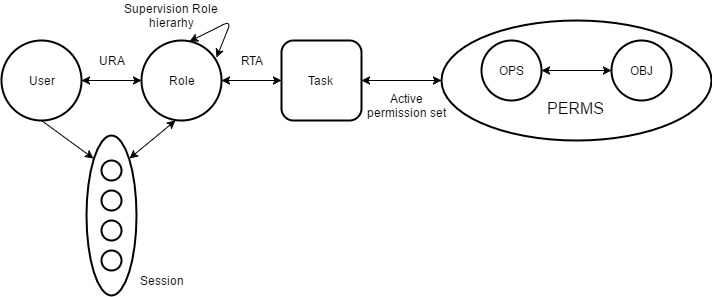
\includegraphics[width=0.7\textwidth, height=0.39\textwidth]{Img/self/TBAC.jpg}
    \caption{TBAC scheme partially adapted from Task-Role Based Dual System Access Control Model\cite{TBAC2}}
\end{figure}


\section{Prototype choices}
The choice of prototypes is primarily steered by the requirements put forward by the system we use as a case study.
The most straightforward choice was to prototype the role based model and the attribute based model as these 2 approaches stand out as most interesting.
However due to the requirements of the application that is being studied, which we  explain in depth in the next chapter, we need a model that allows more fine grained access control.
\\
\\
First of all we implement the attribute enhanced role based access control model.
This model starts from the role based access control model but adds fine grained access control that the original model lacks and that is required for the application being studied.
This is done by adding attributes to the permissions.
Roles hold a special status over the other attributes, where roles have the permissions assigned to them.
These permissions can have conditions associated with them, which use the other attributes.
This model can be extended the same way as role based access control, with hierarchy and constraints, we did not implement this.
\\
\\
The second model we implement is the attribute based access control model, this is a more general approach that does not rely on roles to be associated with rules. 
Instead the policies made are enforced on the complete system, every time someone tries to access an object all rules on that object will be tested.
There will still be roles, but they are one of the attributes that is being used in this model, they are just part of the conditions that are being used.
\\
The role based access control model is not implemented because the basic requirements for the case study we perform require more fine grained access control than role based access control offers.
However the basis of this model is part of the implementation of the attribute enhanced role based access control model.
It is possible to let this model behave as the role based access control model by not using conditions.
We will not prototype organizational units because this approach is mainly to make management easier, which can also be done with other methods which expand on what we already have as a system.
The task role based access control model will also not be prototyped since the added possibilities and complexity are overkill compared to the needs of the project.
All of these models excluded can be part of future work on the subject.